\chapter{Ergebnisse}\label{ch:ergebnisse}

Dieses Kapitel präsentiert die Resultate der Klassifizierungsexperimente und stellt sie in den Kontext der in Abschnitt~\ref{sec:zielsetzung-und-beitrage} formulierten Forschungsfragen und Qualitätsziele. Ziel der Untersuchung ist es, \acp{LLM} auf ihre Fähigkeit zur Identifikation \ac{DSGVO}-kritischer Aktivitäten in \ac{BPMN}-Prozessmodellen zu prüfen. Die folgenden Abschnitte fassen die zentralen Erkenntnisse zusammen, analysieren die Ergebnisse entlang verschiedener Modellkategorien, bewerten die Robustheit und veranschaulichen typische Fehlerbilder anhand von Fallstudien. Abschließend werden die Forschungsfragen beantwortet.

Alle Abbildungen und Tabellen in diesem Kapitel wurden auf Basis der im Evaluationsframework generierten Experimentergebnisse erstellt. Dabei wurden die Ergebnisse aus den einzelnen Experimenten zusammengeführt, sodass sämtliche Modelle gemeinsam verglichen werden können. Die im Evaluationsframework erzeugten Diagramme wurden bewusst nicht direkt übernommen, da sie bei vielen Modellen nur schwer skalieren. Die vollständigen Reports und Rohdaten der einzelnen Experimente können weiterhin dem Repository\footnote{Siehe GitLab Repository: \url{https://gitlab.uni-ulm.de/merten/gripl-master-thesis}} entnommen und über das Evaluationsframework erkundet werden.

\section{Zusammenfassung der Ergebnisse}\label{sec:ueberblick}

Für jedes der 13 untersuchten Modelle wurden fünf unabhängige Läufe mit unterschiedlichen Seeds durchgeführt. Abbildung \ref{fig:results-evaluation-metrics-comparison} visualisiert die mittleren Werte für Precision, Recall, F1-Score und Accuracy jeweils inklusive Standardabweichung über alle Wiederholungen hinweg. Für einen besseren Vergleich sind proprietäre Modelle rot, kleinere Modelle orange und größere Modelle blau eingefärbt. Die Einteilung entspricht der in Kapitel~\ref{ch:modellauswahl} beschriebenen Kategorisierung.

\begin{figure}[h]
    \centering
    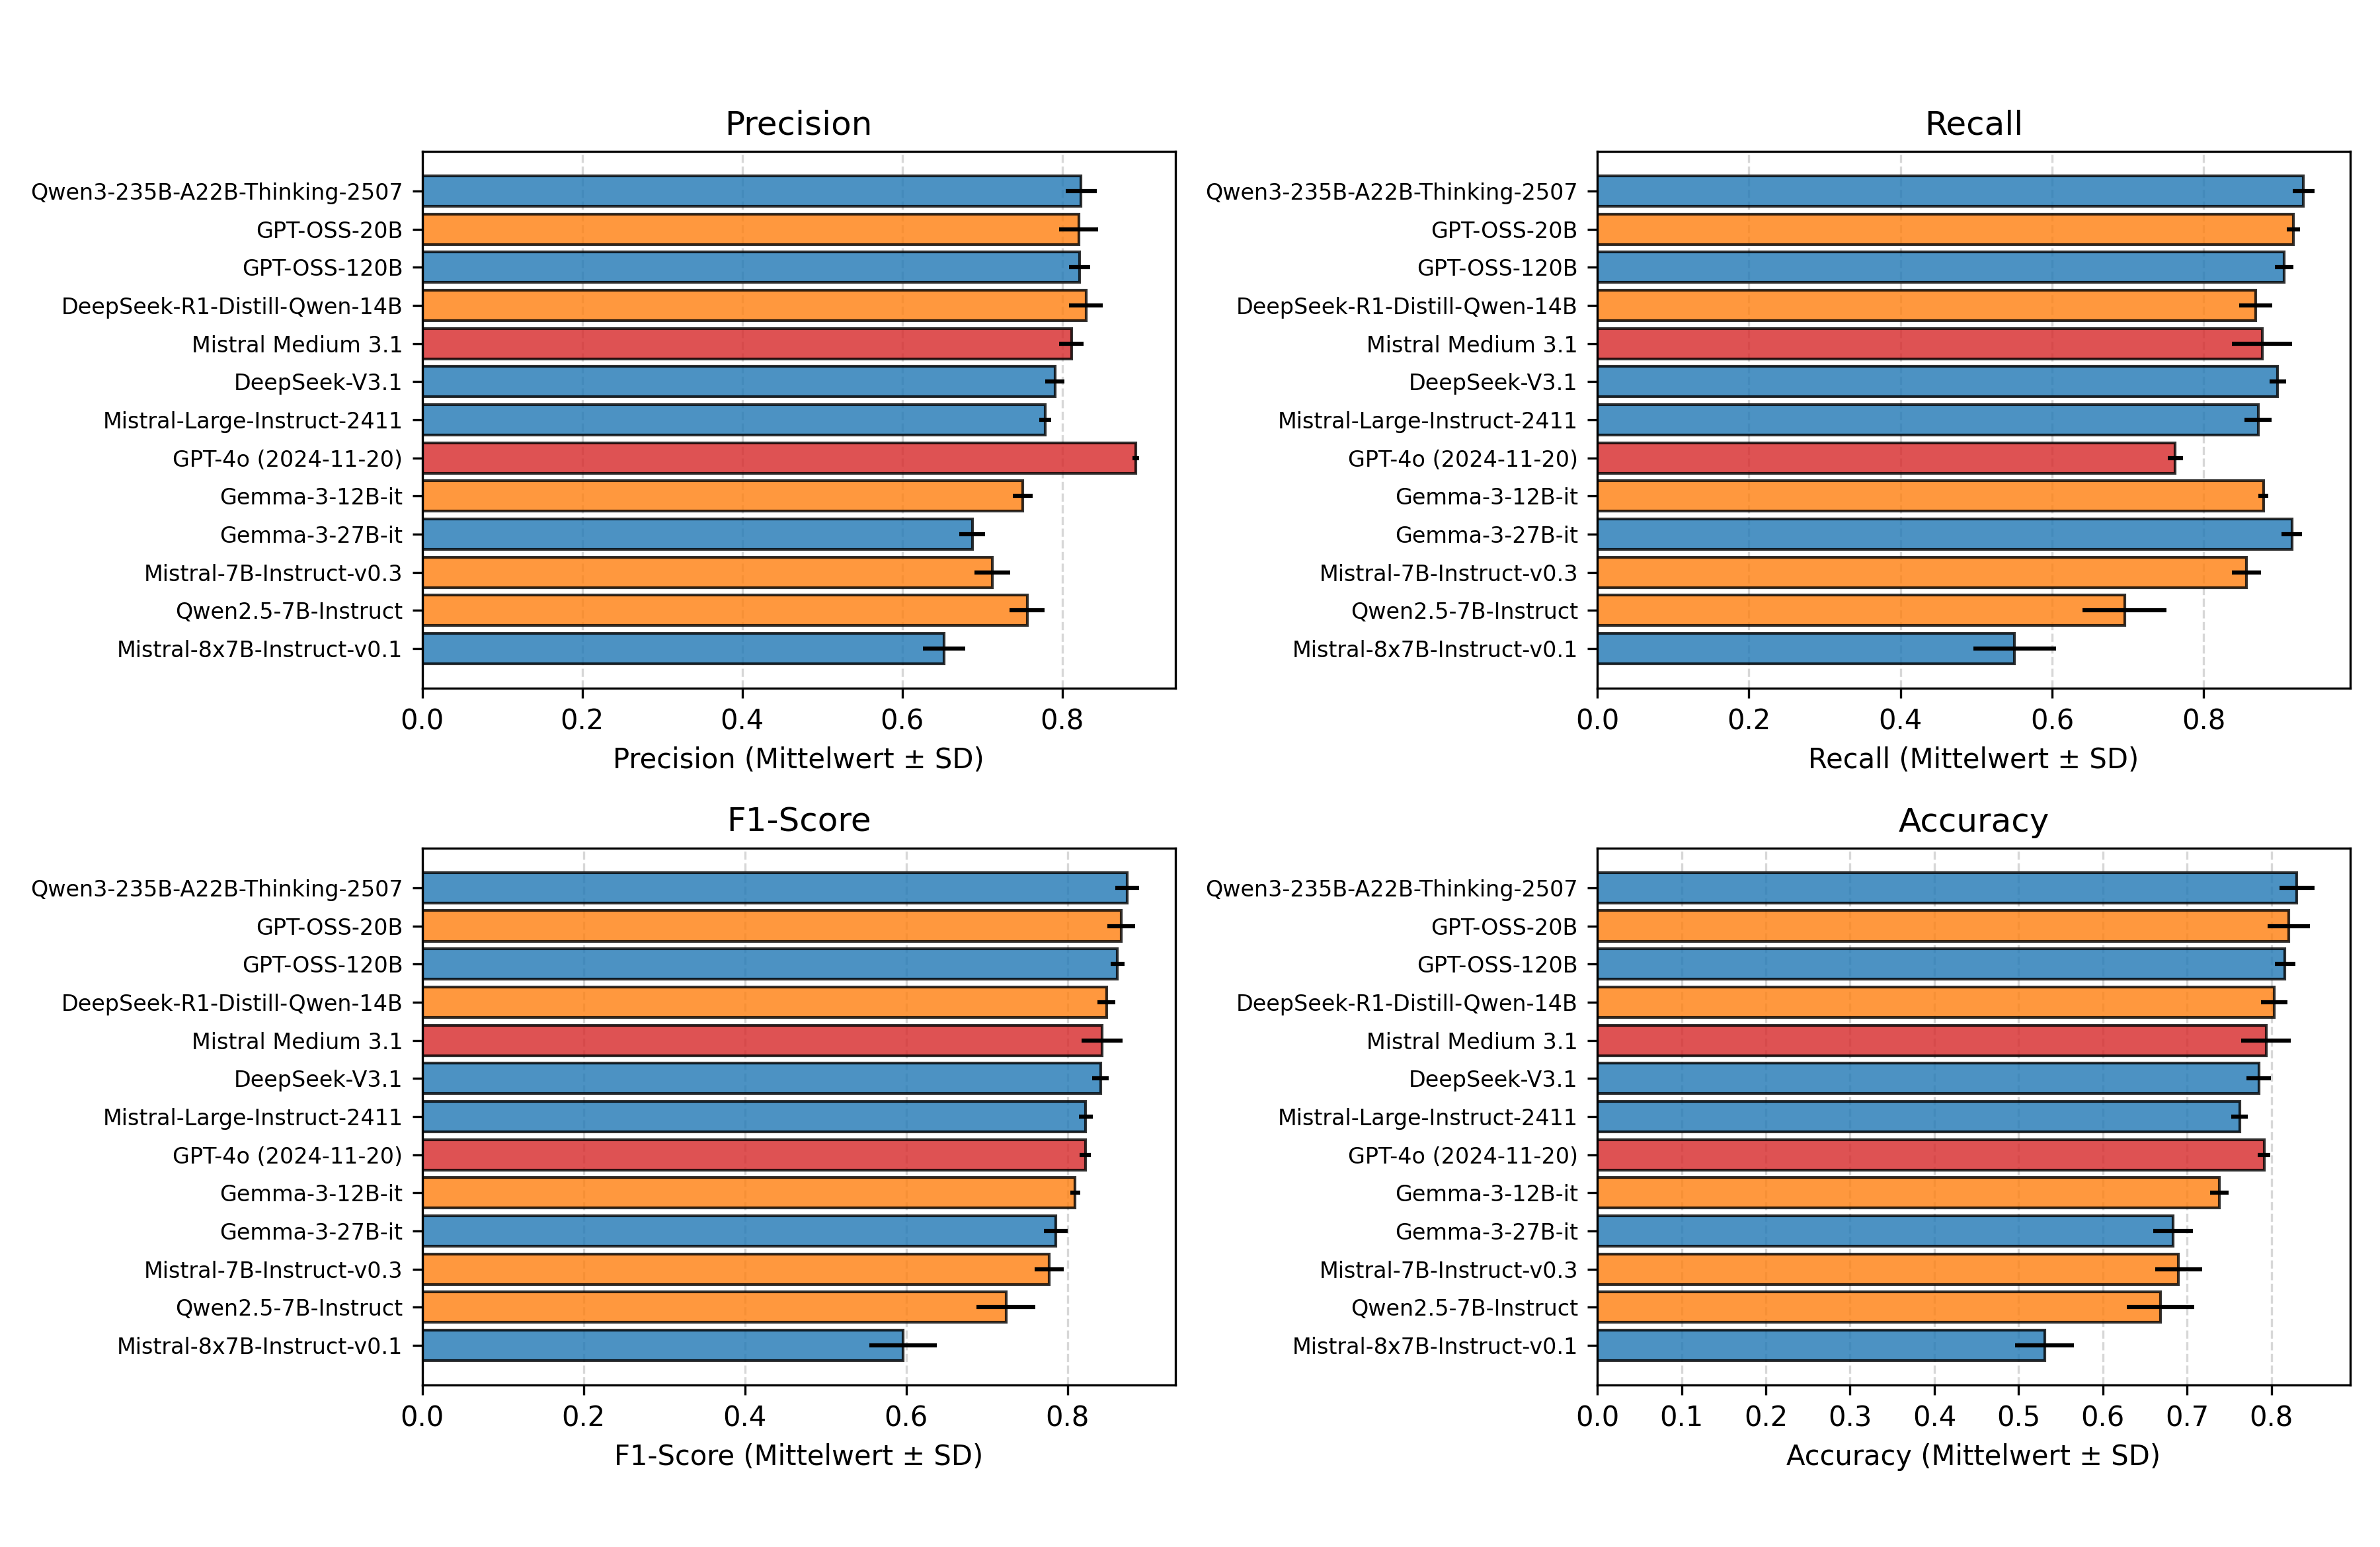
\includegraphics[width=\textwidth]{images/results/evaluation_metrics_comparison}
    \caption{Durchschnittliche Werte für Precision, Recall, F1-Score und Accuracy der untersuchten Modelle über alle Wiederholungen hinweg inklusive Standardabweichung.}
    \label{fig:results-evaluation-metrics-comparison}
\end{figure}

Für die Einordnung der Ergebnisse ist entscheidend, wie Precision und Recall zu interpretieren sind: Ein höherer \emph{Recall} bedeutet, dass ein Modell nur wenige kritische Aktivitäten übersieht (wenige \ac{FN}) und eignet sich damit besonders gut als vorsorgliches \emph{Screening}. Eine höhere \emph{Precision} zeigt dagegen, dass selten unkritische Aktivitäten fälschlich als kritisch markiert werden (wenige \ac{FP}), sodass der manuelle Prüfaufwand sinkt. Der \emph{F1-Score} als harmonisches Mittel aus Precision und Recall fasst beide Perspektiven zu einer Kennzahl zusammen: Er steigt nur dann, wenn \emph{beide} Werte hoch sind, und bestraft Ungleichgewichte (z.\,B. sehr hohe Precision bei niedrigem Recall). Entsprechend setzen die Qualitätsziele in Abschnitt~\ref{sec:qualitatsziele} einen F1-Score $\geq 0{,}80$ als Maß für die kombinierte Screening-Leistung, priorisieren aber den Recall, um das Übersehen kritischer Aktivitäten zu vermeiden. Vor diesem Hintergrund lassen sich die in Abbildung~\ref{fig:results-evaluation-metrics-comparison} sichtbaren Unterschiede zwischen den Modellen einordnen und erklären.

Insgesamt erfüllen neun der dreizehn Modelle den Zielwert eines F1-Scores $\geq 0{,}80$ aus Abschnitt~\ref{sec:qualitatsziele}. Besonders gut schneiden \texttt{Qwen3-235B-A22B-Thinking-2507}, \texttt{GPT-OSS-120B} und \texttt{GPT-OSS-20B} ab, die F1-Scores zwischen $0{,}862$ und $0{,}874$ erreichen. Hervorzuheben ist, dass auch mehrere kleinere Modelle diesen Zielwert überschreiten. Am unteren Ende des Spektrums liegt das europäische \texttt{Mixtral-\linebreak~8x7B-Instruct-v0.1}, das sowohl in Precision als auch in Recall schwach abschneidet und als einziges Modell einen F1-Score deutlich unter $0{,}60$ erzielt.

Die Abbildung zeigt zudem, dass sich die Modelle hinsichtlich Precision und Recall unterschiedlich verhalten. \texttt{GPT-4o} erreicht beispielsweise mit $0{,}892$ die höchste Precision, liegt jedoch beim Recall mit $0{,}762$ unter dem Mindestziel von $0{,}80$ - es würde demnach in der Praxis vergleichsweise viele kritische Aktivitäten übersehen. Umgekehrt erzielt \texttt{Gemma-3-27B-it} einen sehr hohen Recall von $0{,}916$, wird aber durch eine niedrige Precision von $0{,}687$ ausgebremst. Dadurch klassifiziert es viele unkritische Aktivitäten fälschlich als kritisch, was den manuellen Prüfaufwand erhöhen würde. Modelle wie \texttt{Qwen3-235B-A22B-Thinking-2507}, \texttt{GPT-OSS-20B} und \texttt{DeepSeek-R1-Distill-Qwen-14B} bieten eine ausgewogene Balance und zählen deshalb zu den Spitzenreitern.

Tabelle \ref{tab:metrics-overview} fasst alle Metriken mit ihren Mittelwerten und Standardabweichungen tabellarisch zusammen. Für die weitere Analyse werden diese Werte nur noch punktuell zitiert, um Wiederholungen zu vermeiden.

\begin{table}[htbp]
    \centering
    \caption{Aggregierte Mittelwerte und Standardabweichungen der Evaluationsmetriken über alle fünf Wiederholungen hinweg.}
    \label{tab:metrics-overview}
    \begin{adjustbox}{width=\textwidth}
        \begin{tabular}{l r r r r}
            \toprule
            Modell                          & Precision         & Recall            & F1-Score          & Accuracy \\
            \midrule
            DeepSeek-V3.1                   & 0,791 $\pm$ 0,012 & 0,897 $\pm$ 0,011 & 0,841 $\pm$ 0,011 & 0,785 $\pm$ 0,015 \\
            DeepSeek-R1-Distill-Qwen-14B    & 0,829 $\pm$ 0,021 & 0,868 $\pm$ 0,022 & 0,848 $\pm$ 0,011 & 0,803 $\pm$ 0,016 \\
            Gemma-3-12B-it                  & 0,751 $\pm$ 0,013 & 0,879 $\pm$ 0,006 & 0,810 $\pm$ 0,006 & 0,738 $\pm$ 0,011 \\
            Gemma-3-27B-it                  & 0,687 $\pm$ 0,016 & 0,916 $\pm$ 0,014 & 0,785 $\pm$ 0,015 & 0,683 $\pm$ 0,023 \\
            Mistral-7B-Instruct-v0,3        & 0,712 $\pm$ 0,022 & 0,856 $\pm$ 0,019 & 0,777 $\pm$ 0,018 & 0,690 $\pm$ 0,028 \\
            Mixtral-8x7B-Instruct-v0,1      & 0,652 $\pm$ 0,027 & 0,550 $\pm$ 0,054 & 0,596 $\pm$ 0,042 & 0,531 $\pm$ 0,035 \\
            Mistral-Large-Instruct-2411     & 0,779 $\pm$ 0,008 & 0,872 $\pm$ 0,018 & 0,823 $\pm$ 0,008 & 0,762 $\pm$ 0,010 \\
            Mistral Medium 3.1              & 0,811 $\pm$ 0,015 & 0,877 $\pm$ 0,040 & 0,843 $\pm$ 0,025 & 0,794 $\pm$ 0,029 \\
            GPT-OSS-20B                     & 0,820 $\pm$ 0,024 & 0,918 $\pm$ 0,009 & 0,866 $\pm$ 0,017 & 0,821 $\pm$ 0,025 \\
            GPT-OSS-120B                    & 0,822 $\pm$ 0,013 & 0,906 $\pm$ 0,012 & 0,862 $\pm$ 0,009 & 0,816 $\pm$ 0,012 \\
            GPT-4o                          & 0,892 $\pm$ 0,004 & 0,762 $\pm$ 0,010 & 0,822 $\pm$ 0,007 & 0,791 $\pm$ 0,007 \\
            Qwen2.5-7B-Instruct             & 0,756 $\pm$ 0,022 & 0,696 $\pm$ 0,055 & 0,724 $\pm$ 0,037 & 0,668 $\pm$ 0,040 \\
            Qwen3-235B-A22B-Thinking-2507   & 0,824 $\pm$ 0,019 & 0,932 $\pm$ 0,014 & 0,874 $\pm$ 0,015 & 0,830 $\pm$ 0,021 \\
            \bottomrule
        \end{tabular}
    \end{adjustbox}
\end{table}

Neben den zusammengeführten Metriken wurden die 25 Testfälle je Modell auch hinsichtlich der Frage ausgewertet, wie viele Testfälle das Modell bestanden hat. Ein Testfall gilt als bestanden, wenn alle \ac{DSGVO}‑kritischen Aktivitäten korrekt klassifiziert und keine unkritischen Aktivitäten fälschlicherweise als kritisch markiert wurden. Schlägt ein Testfall fehl, liegt mindestens eine Fehlklassifikation (\ac{FP} oder \ac{FN}) vor. Daneben gab es wenige technische Fehler, etwa Parsing‑Fehler oder Timeouts, die selbst nach dem in Abschnitt  \ref{sec:validierung-der-ausgabe} beschriebenen Retry‑Mechanismus nicht behoben werden konnten. Diese technischen Fehler wurden, wie in Abschnitt \ref{sec:scope-und-annahmen} festgehalten, nicht in die Metriken einbezogen und sind hier separat ausgewiesen.

\begin{figure}[htbp]
    \centering
    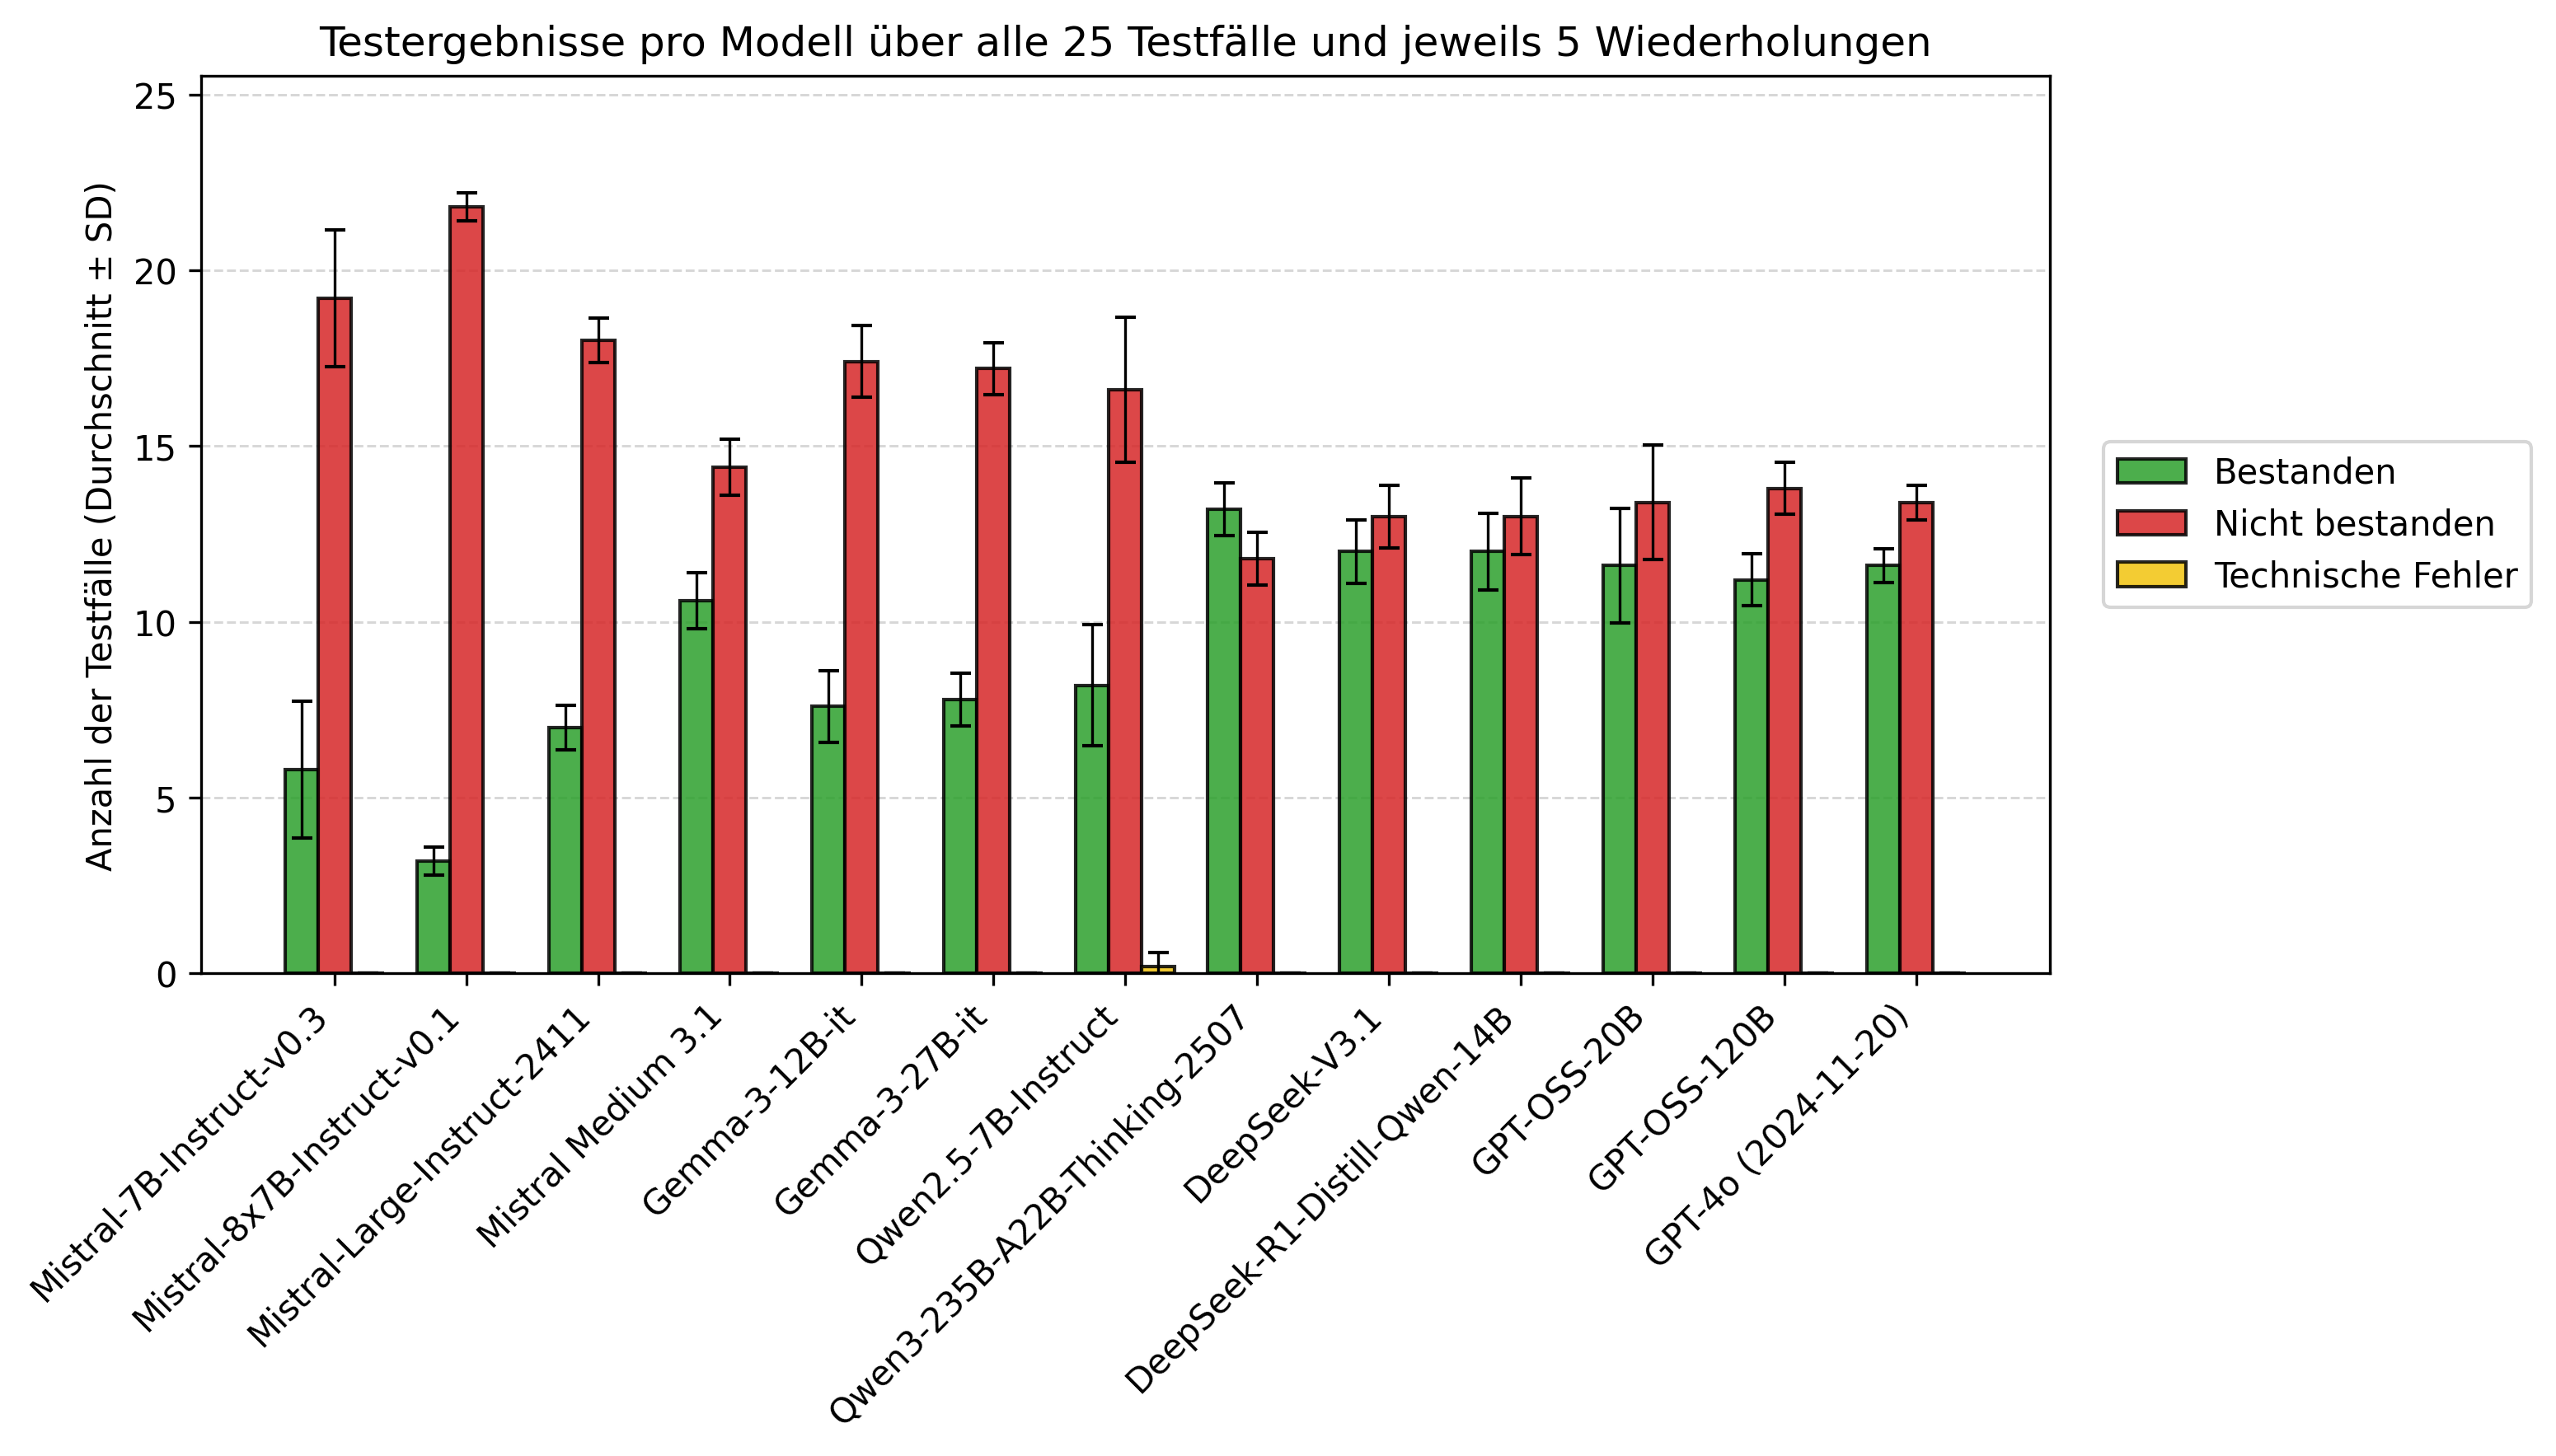
\includegraphics[width=\textwidth]{images/results/evaluation_testcase_outcomes_grouped}
    \caption{Durchschnittliche Testergebnisse pro Modell in Bezug auf die 25 Testfälle über fünf Wiederholungen hinweg.}
    \label{fig:results-testcase-outcomes}
\end{figure}

Wie Abbildung \ref{fig:results-testcase-outcomes} zeigt, korrespondieren die Ergebnisse der Testfälle weitgehend mit den Metriken aus \autoref{tab:metrics-overview}. Modelle wie \texttt{Qwen3-235B-A22B-Thinking-\linebreak~2507}, \texttt{DeepSeek-V3.1} und \texttt{GPT-OSS-20B} bestehen im Durchschnitt fast die Hälfte der Testfälle, während \texttt{Mistral-7B-Instruct-v0.3} und \texttt{Mistral-8x7B-\linebreak~Instruct-v0.1} die meisten Testfälle verfehlen. Auffällig ist, dass \texttt{Qwen2.5-7B-\linebreak~Instruct} als einziges Modell vereinzelte technische Fehler zeigte. Dabei ging es um Parsing-Fehler. Diese treten jedoch selten auf und haben keinen Einfluss auf die berechneten Metriken. Insgesamt bestätigt die Testfallanalyse, dass die leistungsstärksten Modelle nicht nur hohe Metrikwerte erzielen, sondern auch die meisten Testfälle bestehen.
\section{Analyse}\label{sec:analyse}

\begin{itemize}
    \item Aufschlüsselung nach Datensätzen
    \item Aufzeigen sichtbarer Muster
\end{itemize}
\section{Robustheit}\label{sec:robustheit}

Die Robustheit der Modelle wird anhand zweier Kriterien bewertet: der Varianz der F1-Scores über die verschiedenen Seeds und der Anzahl der Retries, die erforderlich waren, um eine formatkorrekte JSON-Antwort von den \acp{LLM} in der Klassifizierungspipeline zu erhalten. Beide Größen geben Aufschluss darüber, wie stabil ein Modell im produktiven Einsatz ist.

Abbildung \ref{fig:results-evaluation-robustness-f1-std} zeigt die Standardabweichungen der F1‑Scores über fünf unabhängige Läufe mit unterschiedlichen Seeds. Die Mehrzahl der Modelle weist Werte von deutlich unter $0{,}02$ auf. Sie liefern damit weitgehend gleiche Ergebnisse, unabhängig vom gewählten Seed, und gelten als stabil. Dazu zählen \texttt{Gemma-3-12B-it}, \texttt{Mistral-Large-Instruct-2411}, \texttt{GPT-OSS-120B} und \texttt{DeepSeek-R1-Distill-\linebreak~Qwen-14B}.

\begin{figure}[h]
    \centering
    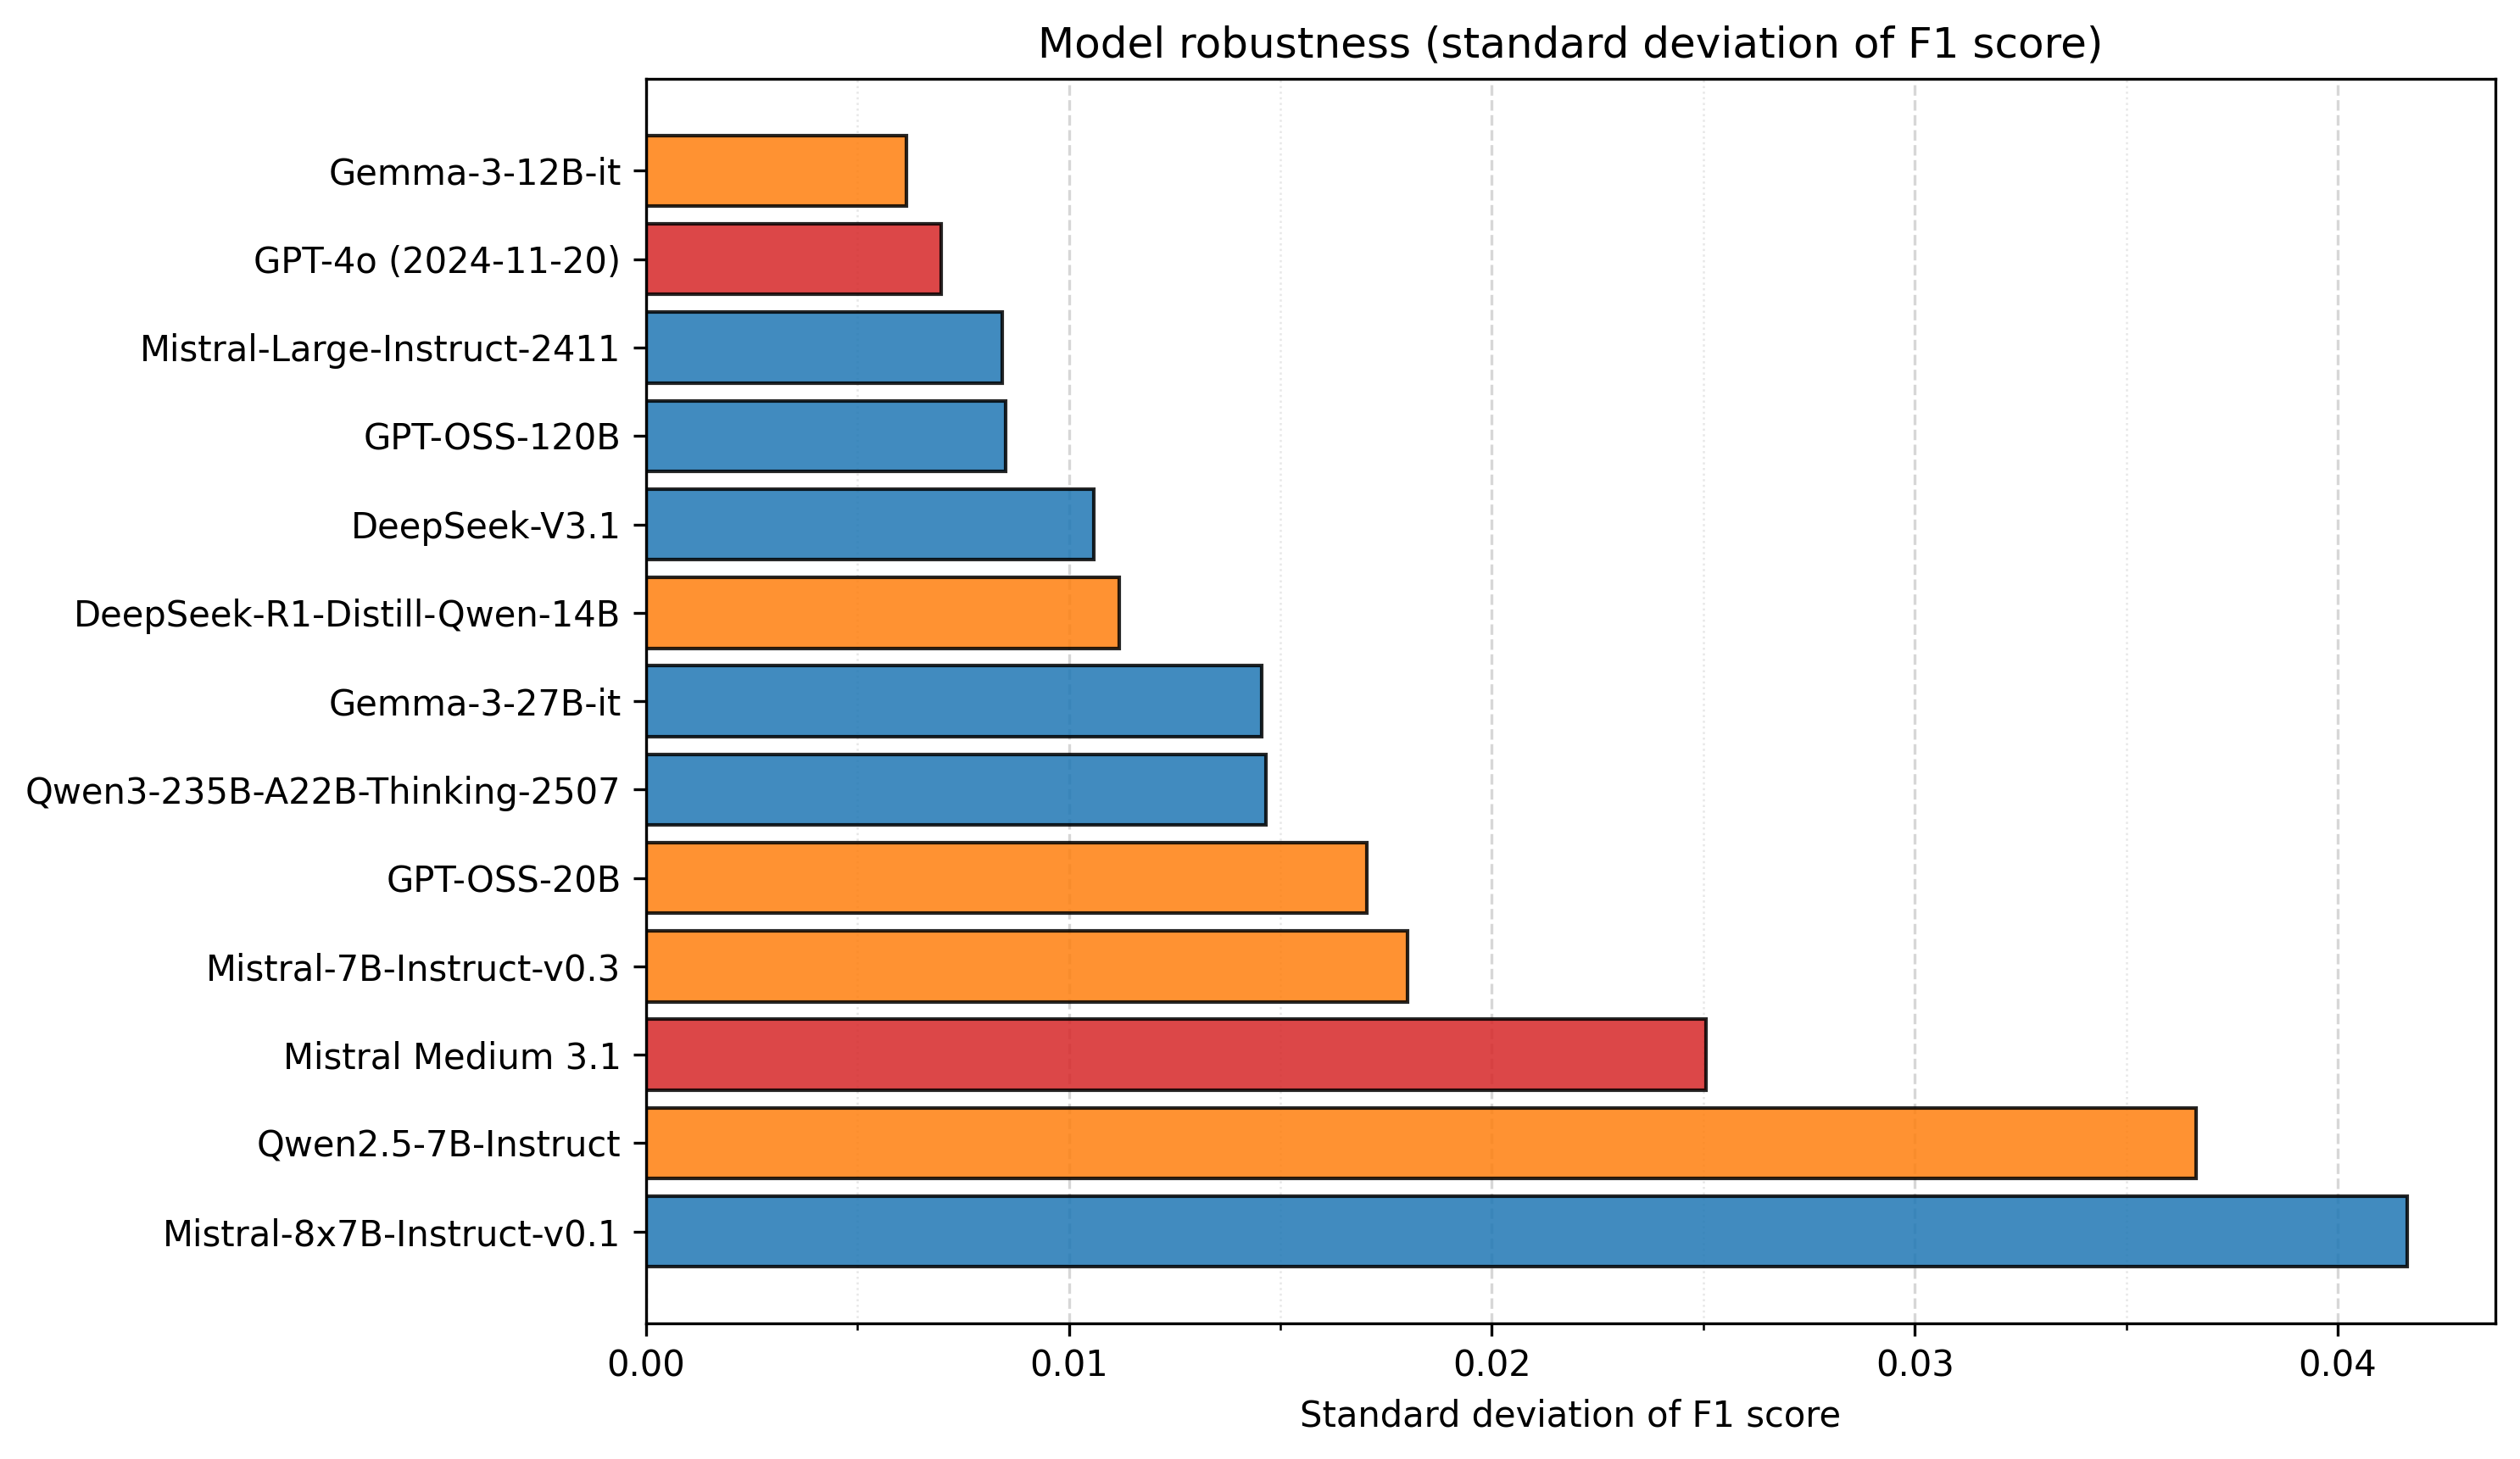
\includegraphics[width=0.7\textwidth]{images/results/evaluation_robustness_f1_std_en}
    \caption{Robustheit der Modelle gemessen an der Standardabweichung des F1-Scores über alle Wiederholungen hinweg.}
    \label{fig:results-evaluation-robustness-f1-std}
\end{figure}

Demgegenüber weisen \texttt{Mistral Medium 3.1}, \texttt{Qwen2.5-7B-Instruct} und vor allem \texttt{Mixtral-8x7B-Instruct-v0.1} mit Standardabweichungen zwischen $0{,}025$ und über $0{,}04$ eine deutlich höhere Varianz auf. Dies bedeutet, dass ihre Leistung stärker vom gewählten Seed abhängt, was die Vergleichbarkeit und Zuverlässigkeit verringert.

Neben der Varianz des F1-Scores ist auch entscheidend, wie oft das Modell nachgefragt werden muss, bis eine gültige JSON-Struktur zurückgegeben wird. Abbildung \ref{fig:results_evaluation_amount_of_retries} zeigt die durchschnittliche Anzahl notwendiger Retries pro Modell über 25 Testfälle. Die meisten Modelle lieferten bereits im ersten Versuch oder nach maximal einem zusätzlichen Aufruf eine korrekte Antwort. Hervorzuheben sind\linebreak~\texttt{DeepSeek-R1-Distill-Qwen-14B}, \texttt{GPT-4o}, \texttt{Gemma-3-12B-it} und \texttt{Mistral-\linebreak~Large-Instruct-2411}, die keinerlei Retries benötigten.

\begin{figure}[h]
    \centering
    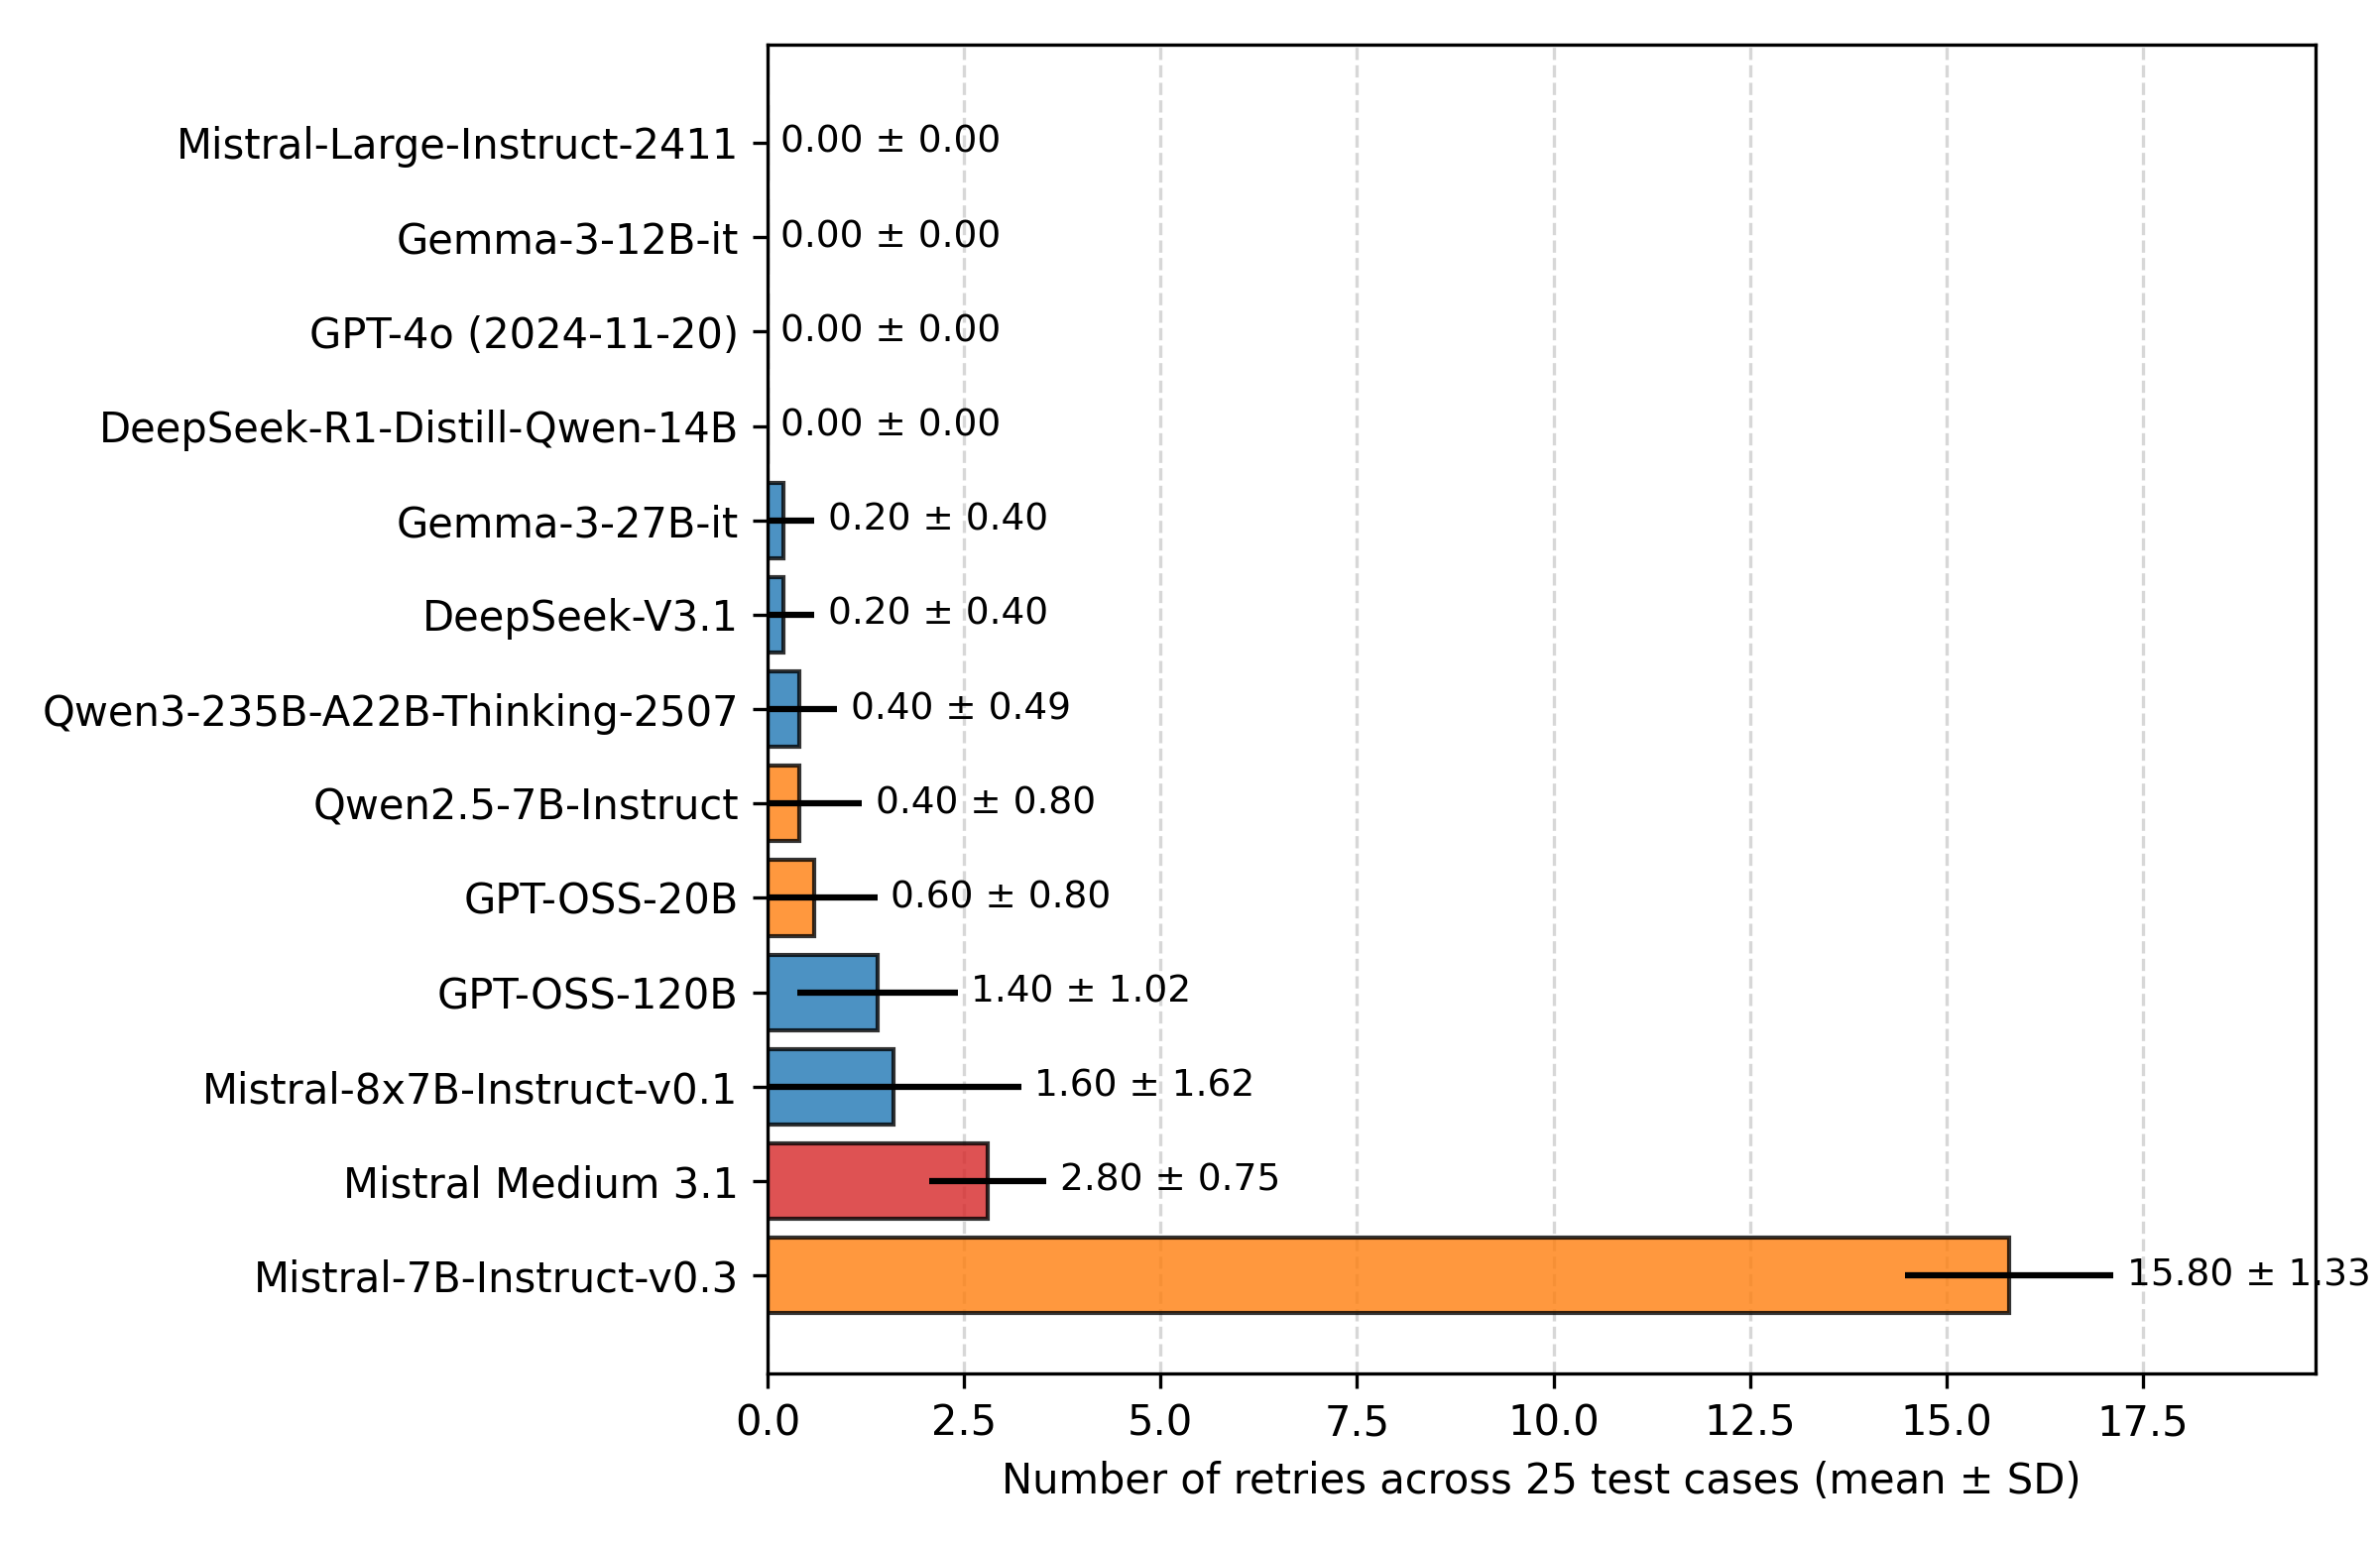
\includegraphics[width=0.7\textwidth]{images/results/evaluation_amount_of_retries_en}
    \caption{Durchschnittliche Anzahl der Retries, die notwendig waren, um für alle 25 Testfälle eine formatkorrekte JSON-Antwort zu erhalten.}
    \label{fig:results_evaluation_amount_of_retries}
\end{figure}

Am anderen Ende des Spektrums steht \texttt{Mistral-7B-Instruct-v0.3}, das im Mittel $15{,}8$ zusätzliche Aufrufe benötigte, was im Durchschnitt etwa $0{,}63$ Retries pro Testfall entspricht. Diese hohe Zahl verdeutlicht, dass das Modell Schwierigkeiten hat, die vorgegebenen Formatierungsregeln zuverlässig einzuhalten.

In Kombination mit der geringen Varianz sind \texttt{Gemma-3-12B-it}, \texttt{Mistral-Large-\linebreak~Instruct-2411} und \texttt{DeepSeek-R1-Distill-Qwen-14B} die robustesten Modelle: Sie liefern konsistente Ergebnisse und halten das Ausgabeschema zuverlässig ein. Modelle wie \texttt{Mistral Medium 3.1}, \texttt{Qwen2.5-7B-Instruct} und \texttt{Mixtral-8x7B-\linebreak~Instruct-v0.1} sind hingegen anfälliger für Schwankungen und erfordern häufiger Wiederholungen.
\section{Fallstudien}\label{sec:fallstudien}

\begin{itemize}
    \item Hier werde ich (wahrscheinlich 2--3) spezifische exemplarische Ergebnisse von Testcases heraussuchen und genauer unter die Lupe nehmen. Was ist hier besonders aufgefallen oder interessant?
    \item Hier kann ich die Bilder mit den Highlights hernehmen
    \item Idealerweise habe ich Beispiele für 1. TN, 2. FP aber plausible Erklärung und 3. FN
\end{itemize}
\section{Antworten auf Forschungsfragen}\label{sec:antworten-auf-forschungsfragen}

Basierend auf den vorstehenden Auswertungen können die in \ref{sec:zielsetzung-und-beitrage} formulierten Forschungsfragen beantwortet werden. Die nachfolgenden Antworten berücksichtigen sowohl die quantitativen Ergebnisse als auch qualitative Beobachtungen aus den Fallstudien und ordnen sie unter berücksichtigung der Qualitätsziele aus Abschnitt \ref{sec:qualitatsziele} ein.

\paragraph{UF1: Wie gut schneiden europäische Modelle im Vergleich zu internationalen Modellen ab?}

Die europäischen Modelle zeigen eine große Spannweite in ihrer Leistungsfähigkeit. Wie in Abschnitt~\ref{sec:qualitatsziele} dargelegt, gelten als Qualitätsziele ein Recall von mindestens $0{,}80$ mit angestrebtem Bereich ab $0{,}85$, eine Precision von mindestens $0{,}75$, ein F1-Score von mindestens $0{,}80$ sowie höchstens $1{,}5$ \acp{FP} je Prozess.

Das proprietäre \texttt{Mistral Medium 3.1} ist mit einem F1-Score von $0{,}843$ und einem Recall von $0{,}877$ das leistungsstärkste \ac{EU}-Modell. Es übertrifft \texttt{GPT-4o} beim F1-Score und beim Recall, liegt jedoch hinter den besten internationalen Modellen. Im Rahmen der Qualitätsziele erfüllt \texttt{Mistral Medium 3.1} alle Kriterien, denn der Recall liegt im angestrebten Bereich, die Precision von $0{,}811$ überschreitet die Untergrenze und der F1-Score liegt über dem Zielwert.

\texttt{Mistral-Large-Instruct-2411} bewegt sich mit Blick auf F1-Score und Recall im Mittelfeld der getesteten Modelle und liegt knapp vor \texttt{GPT-4o}. Die Qualitätsziele werden erreicht, denn der Recall beträgt $0{,}872$ und erreicht das Mindestniveau, die Precision liegt mit $0{,}779$ über der Untergrenze und der F1-Score von $0{,}823$ erfüllt das Ziel.

Das kleine Modell \texttt{Mistral-7B-Instruct-v0.3} erzielt mit F1-Score $0{,}777$ und Recall $0{,}856$ – insbesondere für die Größe – solide Werte und ordnet sich insgesamt im unteren Mittelfeld ein. Das Recall-Ziel wird erreicht, die Precision von $0{,}712$ unterschreitet jedoch die Untergrenze, und der F1-Score bleibt dadurch unter dem Zielwert.

Das \ac{MoE}-Modell \texttt{Mixtral-8x7B-Instruct-v0.1} schneidet mit F1-Score $0{,}596$ und Recall $0{,}550$ deutlich schlechter ab und bildet das Schlusslicht der getesteten Modelle. Sämtliche Zielwerte werden verfehlt, da auch die Precision mit $0{,}652$ unter der Untergrenze liegt.

In jeder Größenklasse finden sich internationale Modelle, die die europäischen Modelle übertreffen. \texttt{Qwen3-235B-A22B-Thinking-2507} erreicht einen Recall von $0{,}932$ und einen F1-Score von $0{,}874$ und liegt damit klar im Zielbereich. \texttt{GPT-OSS-20B} und \texttt{GPT-OSS-120B} erfüllen mit Recall $0{,}918$ beziehungsweise $0{,}906$ und F1-Score $0{,}866$ beziehungsweise $0{,}862$ sämtliche Kriterien. \texttt{GPT-4o} erfüllt mit Precision $0{,}892$ und F1-Score $0{,}822$ die entsprechenden Zielwerte, unterschreitet jedoch das Recall-Mindestniveau mit $0{,}762$.

Damit lässt sich festhalten, dass die internationalen Modelle im Mittel eine höhere Klassifikationsqualität bieten. \ac{EU}-Modelle können vor allem durch ihre datenschutzfreundliche Bereitstellung und ihren Standortvorteil punkten. Leistungsmäßig erfüllen \texttt{Mistral Medium 3.1} und \texttt{Mistral-Large-Instruct-2411} die Qualitätsziele, während \texttt{Mistral-7B-Instruct-v0.3} und \texttt{Mixtral-8x7B-Instruct-\linebreak~v0.1} diese nicht vollständig erreichen.

\paragraph{UF2: Wie unterschieden sich große und kleine Modelle in ihrer Leistungsfähigkeit?}

Die Gegenüberstellung kleiner Modelle mit $\leq 25B$ Parametern und großer Modelle mit $> 25B$ Parametern ergab kaum Unterschiede im Durchschnitt. Der mittlere F1-Score liegt mit $0{,}805$ bei den kleinen und $0{,}806$ bei den großen Modellen praktisch gleichauf. Ohne das deutlich unterdurchschnittliche \texttt{Mixtral-\linebreak~8x7B-Instruct-v0.1} steigt der Durchschnitt der großen Modelle auf $0{,}836$, was zeigt, dass größere Modelle tendenziell bessere Leistungen erbringen können. Die Recall-Werte der kleinen Modelle von durchschnittlich $0{,}843$ übertreffen die der großen Modelle von $0{,}839$ leicht, während Precision und Accuracy in beiden Gruppen vergleichbar sind. Auffällig ist die höhere Varianz der großen Modelle: die Standardabweichung des F1-Scores beträgt $0{,}089$, bei den kleinen lediglich $0{,}057$. Dies ist vor allem auf das Ausreißermodell \texttt{Mixtral-8x7B-Instruct-v0.1} zurückzuführen. Bei den Bestwerten liegen die Gruppen einigermaßen dicht beieinander: das beste kleine Modell \texttt{GPT-OSS-20B} erzielt einen F1-Score von $0{,}866$ und einen Recall von $0{,}918$, während das beste große Modell \texttt{Qwen3-235B-A22B-Thinking-\linebreak~2507} einen F1-Score von $0{,}874$ und einen Recall von $0{,}932$ erreicht.

Die Analyse zeigt, dass die Modellgröße allein kein entscheidender Faktor für die Klassifikationsleistung ist. Vielmehr sind Trainingsdaten, Feinabstimmung und Architektur entscheidender. Leistungsfähige kleine Modelle können mit den großen mithalten und sind im praktischen Einsatz ressourcenschonender.

\paragraph{UF3: Welche Open-Source-Modelle (insbesondere aus der EU) erzielen die besten Ergebnisse?}

Unter den offenen Modellen erzielen \texttt{Qwen3-235B-A22B-\linebreak~Thinking-2507}, \texttt{GPT-OSS-20B} und \texttt{DeepSeek-R1-Distill-Qwen-14B} die besten Ergebnisse. \texttt{Qwen3-235B-A22B-Thinking-2507} erreicht mit einem F1-Score von $0{,}874$, einem Recall von $0{,}932$ und einer Precision von $0{,}824$ den Spitzenplatz. \texttt{GPT-OSS-20B} folgt mit F1 $0{,}866$, Recall $0{,}918$ und Precision $0{,}820$. Auch das kleinere \texttt{DeepSeek-R1-Distill-Qwen-14B} überzeugt mit einem F1-Score von $0{,}848$ und einer Precision von $0{,}829$. Diese Modelle übertreffen die proprietären Benchmarks und erfüllen die Qualitätsziele klar.

Die europäischen Open-Source-Modelle weisen hingegen ein heterogenes Leistungsbild auf. \texttt{Mistral-Large-Instruct-2411} ist mit einem F1-Score von $0{,}823$ und einer Precision von $0{,}779$ das leistungsstärkste offene EU-Modell und erfüllt alle Qualitätsziele. \texttt{Mistral-7B-Instruct-v0.3} erreicht zwar einen Recall von $0{,}856$, bleibt mit einer Precision von $0{,}712$ und F1-Score von $0{,}777$ aber unter den Zielwerten. \texttt{Mixtral-8x7B-Instruct-v0.1} schneidet mit einem F1-Score von $0{,}596$ und Recall von $0{,}550$ deutlich schlechter ab und verfehlt alle Ziele.

Insgesamt dominieren bei den Open-Source-Modellen die chinesischen Qwen-\linebreak~Varianten und die GPT-OSS-Modelle das Feld, während europäische Modelle im Schnitt hinter den internationalen Spitzenreitern zurückbleiben.

\paragraph{UF4: Wie gut schneiden Open-Source-Modelle gegenüber kommerziellen Modellen wie GPT-4o ab?}

Der Vergleich zeigt, dass mehrere Open-Source-Modelle die kommerziellen Vertreter in der Klassifikationsqualität übertreffen. Zu den proprietären Modellen im Vergleichsfeld zählen \texttt{GPT-4o} und das europäische \texttt{Mistral Medium 3.1}. \texttt{Mistral Medium 3.1} erreicht einen F1-Score von $0{,}843$, einen Recall von $0{,}877$ und eine Precision von $0{,}811$ und liegt damit vor \texttt{GPT-4o}, das einen F1-Score von $0{,}822$, einen Recall von $0{,}762$ und eine sehr hohe Precision von $0{,}892$ erzielt.

Unter den offenen Modellen führen \texttt{Qwen3-235B-A22B-Thinking-2507} mit einem F1-Score von $0{,}874$, einem Recall von $0{,}932$ und einer Precision von $0{,}824$ sowie \texttt{GPT-OSS-20B} mit einem F1-Score von $0{,}866$, einem Recall von $0{,}918$ und einer Precision von $0{,}820$. Das kleinere \texttt{DeepSeek-R1-Distill-Qwen-14B} liegt beim F1-Score mit $0{,}848$ ebenfalls über \texttt{GPT-4o}, erreicht jedoch nicht dessen außergewöhnlich hohe Precision. Gleichzeitig ist die Spannweite innerhalb der Open-Source-Kategorie größer, wie das schwache Abschneiden von \texttt{Mixtral-8x7B-\linebreak~Instruct-v0.1}.

Insgesamt zeigen hochwertige Open-Source-Modelle die stärkste Balance aus hohem Recall und hohem F1-Score und erfüllen die Qualitätsziele klar, während\linebreak~\texttt{GPT-4o} durch exzellente Precision überzeugt, aber aufgrund des niedrigen Recalls häufiger kritische Aktivitäten übersieht. \texttt{Mistral Medium 3.1} belegt, dass ein kommerzielles \ac{EU}-Modell die Ziele ebenfalls erfüllt und im F1-Score und Recall vor \texttt{GPT-4o} liegt.

Auf Basis der durchgeführten Experimente, Analysen und Antworten auf die Unterfragen lässt sich die Hauptforschungsfrage beantworten im Folgenden beantworten.

\paragraph{FF1: Wie zuverlässig identifizieren LLM DSGVO-kritische Aktivitäten in BPMN-Prozessmodellen?}

Die Ergebnisse zeigen, dass moderne \acp{LLM} \ac{DSGVO}-\linebreak~kritische Aktivitäten mit hoher Zuverlässigkeit erkennen können. Insgesamt erfüllten neun von dreizehn Modellen den F1-Score-Zielwert von mindestens $0{,}80$, darunter auch mehrere kleinere Modelle. Die besten Modelle – \texttt{Qwen3-235B-A22B-\linebreak~Thinking-2507}, \texttt{GPT-OSS-20B}, \texttt{DeepSeek-R1-Distill-Qwen-14B} und \texttt{Mistral Medium 3.1} – erzielten F1-Scores zwischen $0{,}843$ und $0{,}874$ sowie Recall-Werte von $0{,}868$ bis $0{,}932$, überschritten damit deutlich die aus der Literatur abgeleiteten Referenzwerte und erfüllten die Qualitätsziele. Gleichzeitig gibt es Modelle wie \texttt{Mixtral-8x7B-Instruct-v0.1} und \texttt{Qwen2.5-7B-Instruct}, die mit F1-Scores unter $0{,}60$ beziehungsweise $0{,}73$ und Recall unter $0{,}70$ deutlich abfallen.

Die Robustheitsanalyse zeigt, dass die meisten Modelle eine sehr geringe Varianz zwischen verschiedenen Seeds aufweisen: die Standardabweichung des F1-Scores liegt oft unter $0{,}02$. Modelle wie \texttt{Gemma-3-12B-it}, \texttt{Mistral-Large-\linebreak~Instruct-2411} und \texttt{DeepSeek-R1-Distill-Qwen-14B} benötigten zudem keine Retries, um eine korrekte JSON-Antwort zu liefern, was ihre Zuverlässigkeit unterstreicht. Dagegen reagieren \texttt{Mistral Medium 3.1}, \texttt{Qwen2.5-7B-Instruct} und vor allem \texttt{Mixtral-8x7B-Instruct-v0.1} empfindlicher auf den Seed und erfordern bei Formatierung der Ausgabe teilweise zahlreiche Wiederholungen.

Die Fallstudien verdeutlichen typische Fehlerbilder. Im Testfall \enquote{Sales Warehouse} erkannte \texttt{Qwen3-235B-A22B-Thinking-2507} alle kritischen Aktivitäten, markierte aber zusätzlich das Versenden eines Produkts als kritisch, weil das Modell die Nutzung der Kundenadresse als potenzielle Datenverarbeitung interpretierte, während bei der Modellierung lediglich an einen logistischen Schritt gedacht war. Dieses \ac{FP} ist angesichts des angestrebten hohen Recalls akzeptabel. Im Szenario \enquote{Marketing-Kampagne} identifizierte \texttt{GPT-OSS-20B} die anonymisierte Auswertung von Klickraten fälschlich als kritisch, da die notwendigen Kontextinformationen im \ac{BPMN}-Modell fehlten. Umgekehrt zeigte der Testfall \enquote{Karten-App – Standort erfassen}, dass \texttt{Mistral-Large-Instruct-2411} trotz vorhandener Datenassoziationen die zweite Aktivität \enquote{Route berechnen} nicht als kritisch markierte. Dieses \ac{FN} widerspricht dem Hauptziel eines maximalen Recalls und weist auf Schwächen bei der Erkennung von Datenflüssen über mehrere Schritte hin.

Zusammenfassend lässt sich festhalten, dass \acp{LLM} \ac{DSGVO}-kritische Aktivitäten in \ac{BPMN}-Prozessmodellen zuverlässig identifizieren können, sofern hochwertige Modelle eingesetzt werden. Die Top-Modelle erfüllen die definierten Qualitätsziele mit Recall-Werten über $0{,}90$ und akzeptabler Precision, die Zahl der \ac{FP} pro Prozess bleibt moderat. Dennoch sind eine sorgfältige Modellwahl und eine nachgelagerte menschliche Prüfung ratsam, um die verbleibenden \acp{FP} und \ac{FN} zu adressieren und die Ergebnisse in den jeweiligen Anwendungskontext einzuordnen.
